
\hypertarget{menu_web}{}
\section{Web}
\index{web menu}

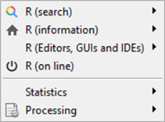
\includegraphics[scale=0.50]{./res/menu_web.png}\\

\begin{scriptsize}
  \begin{tabularx}{\textwidth}{>{\hsize=0.3\hsize}X>{\hsize=0.7\hsize}X}\\
    \hline
    \textbf{Option} & \textbf{Description} \\
    \hline
    R (search) & \textit{\href{\#menu\_web\_rsearch}{See options ...}} \\
    R (information) & \textit{\href{\#menu\_web\_rinformation}{See options ...}} \\
    R (Editors, GUIs and IDEs) & \textit{\href{\#menu\_web\_rguis}{See options ...}} \\
    R (online) & Opens URL \href{https://rdrr.io/snippets/}{rdrr.io} \\
    Statistics & \textit{\href{\#menu\_web\_statistics}{See options ...}} \\
    Processing & \textit{\href{\#menu\_web\_processing}{See options ...}} \\
    \hline
  \end{tabularx}
\end{scriptsize}


\hypertarget{menu_web_rsearch}{}
\subsection{R (search)}
\index{web menu!R search}

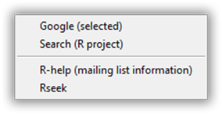
\includegraphics[scale=0.50]{./res/menu_web_rsearch.png}\\

\begin{scriptsize}
  \begin{tabularx}{\textwidth}{>{\hsize=0.5\hsize}X>{\hsize=0.7\hsize}X}\\
    \hline
    \textbf{Option} & \textbf{Description} \\
    \hline
    Google (selected) & Opens URL \href{http://www.google.com/webhp?domains=r-project.org\&sitesearch=r-project.org\&btnG=Google+Search}{Google} and lists the results associated with the word under the cursor or selected text \\
    Search (R project) & Opens URL \href{https://search.r-project.org/}{Search R project} \\
    R-help (mailing list information) & Opens URL \href{http://www.mail-archive.com/r-help@stat.math.ethz.ch/info.html}{r-help} \\
    Rseek & Opens URL \href{http://www.rseek.org/}{Rseek} \\
    \hline
  \end{tabularx}
\end{scriptsize}


\hypertarget{menu_web_rinformation}{}
\subsection{R (information)}
\index{web menu!R information}

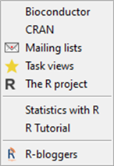
\includegraphics[scale=0.50]{./res/menu_web_rinformation.png}\\

\begin{scriptsize}
  \begin{tabularx}{\textwidth}{>{\hsize=0.3\hsize}X>{\hsize=0.7\hsize}X}\\
    \hline
    \textbf{Option} & \textbf{Description} \\
    \hline
    Bioconductor & Opens URL \href{http://www.bioconductor.org/}{Bioconductor project} \\
    CRAN & Opens URL \href{http://cran.r-project.org/}{The Comprehensive R Archive Network} \\
    Mailing lists & Opens URL \href{https://www.r-project.org/mail.html}{Mailing Lists} \\
    MRAN & Opens URL \href{http://mran.microsoft.com/}{Microsoft R Application Network} \\
    Task views & Opens URL \href{http://cran.r-project.org/web/views/}{CRAN Task Views} \\
    The R project & Opens URL \href{http://www.r-project.org}{The R Project for Statistical Computing} \\
    Statistical with R & Opens URL \href{http://zoonek2.free.fr/UNIX/48\_R/all.html}{Statistical with R} \\
    R tutorial & Opens URL \href{http://www.r-tutor.com/}{R tutorial} \\
    \hline
  \end{tabularx}
\end{scriptsize}


\hypertarget{menu_web_rguis}{}
\subsection{R (Editors, Gui's and IDEs)}
\index{web menu!R Editors}
\index{web menu!R GUIs}
\index{web menu!R IDEs}

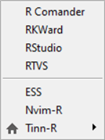
\includegraphics[scale=0.50]{./res/menu_web_rguis.png}\\

\begin{scriptsize}
  \begin{tabularx}{\textwidth}{>{\hsize=0.3\hsize}X>{\hsize=0.7\hsize}X}\\
    \hline
    \textbf{Option} & \textbf{Description} \\
    \hline
    R Comander & Opens URL \href{http://socserv.socsci.mcmaster.ca/jfox/Misc/Rcmdr/index.html}{The R Commander: A Basic-Statistics GUI for R} \\
    RKWard & Opens URL \href{https://rkward.kde.org/}{RKWard} \\
    RStudio & Opens URL \href{http://www.rstudio.com/}{RStudio} \\
    RTVS & Opens URL \href{http://microsoft.github.io/RTVS-docs/}{R Tools for Visual Studio} \\
    ESS & Opens URL \href{http://ess.r-project.org/}{Emacs Speaks Statistics (ESS)} \\
    Nvim-R & Opens URL \href{http://www.vim.org/scripts/script.php?script\_id=2628}{Nvim-R: Plugin to work with R} \\
    Tinn-R & \textit{\href{\#menu\_web\_tinnr}{See options ...}} \\
    \hline
  \end{tabularx}
\end{scriptsize}


\hypertarget{menu_web_tinnr}{}
\subsection{Tinn-R}
\index{web menu!Tinn-R}

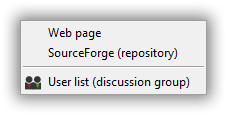
\includegraphics[scale=0.50]{./res/menu_web_tinnr.png}\\


\begin{scriptsize}
  \begin{tabularx}{\textwidth}{>{\hsize=0.3\hsize}X>{\hsize=0.7\hsize}X}\\
    \hline
    \textbf{Option} & \textbf{Description} \\
    \hline
    Web page & Opens URL \href{https://tinn-r.org/en/}{Web page of Tinn-R project} \\
    SourceForge (repository) & Opens URL \href{http://sourceforge.net/projects/tinn-r}{Sourceforge.net Tinn-R} \\
    SciViews (old web page) & Opens URL \href{http://www.sciviews.org/Tinn-R/}{SciViews Tinn-R} \\
    \hline
  \end{tabularx}
\end{scriptsize}


\hypertarget{menu_web_statistics}{}
\subsection{Statistics}
\index{web menu!statistics}

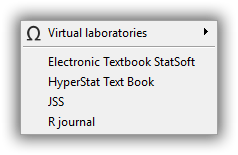
\includegraphics[scale=0.50]{./res/menu_web_statistics.png}\\

\begin{scriptsize}
  \begin{tabularx}{\textwidth}{>{\hsize=0.5\hsize}X>{\hsize=0.7\hsize}X}\\
    \hline
    \textbf{Option} & \textbf{Description} \\
    \hline
    Virtual laboratories & \textit{\href{\#menu\_web\_statistics\_virtuallabs}{See options ...}} \\
    HyperStat Text Book & Opens URL \href{http://davidmlane.com/hyperstat/index.html}{HyperStat Text Book} \\
    JSS & Opens URL \href{http://www.jstatsoft.org/}{Journal of Statistical Software} \\
    R Journal & Opens URL \href{http://journal.r-project.org}{R Journal} \\
    \hline
  \end{tabularx}
\end{scriptsize}


\hypertarget{menu_web_statistics_virtuallabs}{}
\subsubsection{Virtual laboratories}\\
\index{web menu!statistics virtual labs}

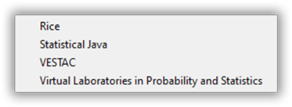
\includegraphics[scale=0.50]{./res/menu_web_statistics_virtuallabs.png}\\

\begin{scriptsize}
\begin{tabularx}{\textwidth}{>{\hsize=0.3\hsize}X>{\hsize=0.7\hsize}X}\\
    \hline
    \textbf{Option} & \textbf{Description} \\
    \hline
    Rice & Opens URL \href{http://onlinestatbook.com/rvls.html}{Rice Virtual Lab in Statistics} \\
    Statistical Java & Opens URL \href{http://www.causeweb.org/repository/statjava/}{Statistical Java} \\
    VESTAC & Opens URL \href{http://lstat.kuleuven.be/newjava/vestac/}{Java Applets for Visualization of Statistical Concepts} \\
    Virtual Laboratories in Probability and Statistics & Opens URL \href{http://www.math.uah.edu/stat/}{Virtual Laboratories in Probability and Statistics} \\
    \hline
  \end{tabularx}
\end{scriptsize}


\newpage
\hypertarget{menu_web_processing}{}
\subsection{Processing}
\index{web menu!processing}

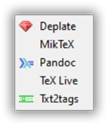
\includegraphics[scale=0.50]{./res/menu_web_processing.png}\\

\begin{scriptsize}
  \begin{tabularx}{\textwidth}{>{\hsize=0.3\hsize}X>{\hsize=0.7\hsize}X}\\
    \hline
    \textbf{Option} & \textbf{Description} \\
    \hline
    Deplate & Opens URL \href{http://deplate.sourceforge.net/index.php}{Sourceforge.net Deplate} \\
    MikTeX & Opens URL \href{http://miktex.org/}{MiKTeX project page} \\
    Pandoc & Opens URL \href{http://johnmacfarlane.net/pandoc/}{Pandoc (a universal document converter)} \\
    TeX Live & Opens URL \href{https://tug.org/texlive/}{TeX Live project page} \\
    Txt2tags & Opens URL \href{http://txt2tags.sourceforge.net/}{Txt2tags ONE source, MULTI targets} \\
    \hline
  \end{tabularx}
\end{scriptsize}
